%\documentclass[11pt,a4paper]{article}
%\documentclass[11pt,a4paper]{scrartcl}
\documentclass[11pt,a4paper,oneside]{book}
\usepackage[british,UKenglish,USenglish,english,american]{babel}
%\usepackage[a4paper, total={16cm, 23cm}]{geometry}
\usepackage[tmargin = 1in,bmargin = 1in,lmargin = 0.75in,rmargin = 
0.75in]{geometry}
\usepackage{tikz}
\usepackage{graphicx}
\usepackage{pgfplots}
\pgfplotsset{width=12cm,compat=1.9}
\usepackage{xcolor}
\usepackage{chemmacros}
\usepackage{chemfig}
%\usepackage{ghsystem}
\usechemmodule{redox}
%\usepackage{chemnum}
%\usepackage{bohr}
%\usepackage{elements}
%\usepackage{endiagram}
%\usepackage{modiagram}
%\usepackage{chemgreek}
%\usepackage{mhchem}
\usepackage{esint}
\usepackage{tabularray}
\usepackage{makeidx}
\usepackage{epstopdf}
\usepackage{amssymb}
\usepackage{mathrsfs}
%\usepackage{minted}
\usepackage{bm}
\usepackage{amsmath}
\usepackage{enumitem}
\usepackage[english]{varioref}
\usepackage[english]{babel}
\usepackage{lipsum}
\usepackage{fancyhdr}
\pagestyle{fancy} 
\usepackage{float}
\usepackage{empheq}
\usepackage[framemethod=tikz]{mdframed}
\usepackage{epstopdf}
\numberwithin{equation}{section}
\usepackage{eso-pic}
\usepackage{calc}
\usepackage{nccmath}
\usepackage{caption}
\usepackage{subcaption}
\usepackage{gensymb}
\usepackage{amsfonts,amsthm,epsfig,epstopdf,titling,url,array}
\usepackage{siunitx}
\sisetup{input-digits = 0123456789\pi}
\usepackage[symbol]{footmisc}
\usepackage{multicol}
\usepackage{boondox-cal}
\DeclareSIUnit\atm{atm}
\setcounter{secnumdepth}{3}
\setcounter{tocdepth}{3}
\usepackage{booktabs}
\usepackage{blindtext}
\usepackage{changepage}
% \usepackage{draftwatermark}
% \SetWatermarkText{DRAFT}
% \SetWatermarkScale{5}

\DeclareSIUnit\atm{atm}

\pagestyle{fancy} 
\fancypagestyle{firstpage}{
\rhead{
%	\begin{picture}(0,0) 
%			\put(-30,0){\includegraphics[width=1cm]{figures/MCI_4C_bw.eps}} 
%	\end{picture}
}
}
\fancyhead[L]{\slshape\nouppercase{\leftmark}}
\chead{}
\rhead{
%	\begin{picture}(0,0) 
%		\put(-30,0){\includegraphics[width=1cm]{figures/MCI_4C_bw.eps}} 
%	\end{picture}
}
\lfoot{\textit{}}
\cfoot{-\ \thepage\ -}
\rfoot{\textit{}}

\DeclareMathOperator{\rank}{rank}
\DeclareMathOperator{\atantwo}{atan2}
\DeclareMathOperator{\spn}{span}

\renewcommand{\headrulewidth}{0.4pt}
\renewcommand{\footrulewidth}{0.4pt}
\newcommand{\abs}[1]{\left|#1\right|}
\definecolor{mycolor1}{rgb}{0.97, 0.97, 0.97}
\definecolor{mycolor2}{rgb}{0.97, 0.97, 0.97}
\definecolor{tableShade}{gray}{0.9}
\newcommand{\sign}{\text{sign}}
\newcommand{\centered}[1]{\begin{tabular}{@{}l@{}} #1 \end{tabular}}
\theoremstyle{it}
\newtheorem{defn}{Definition}[chapter]
\newtheorem{assumption}{Assumption}[chapter]
\newtheorem{thm}{Theorem}[chapter]
\newtheorem{lemma}{Lemma}[chapter]
\newtheorem{corollary}{Corollary}[chapter]
\theoremstyle{definition}
%\theoremstyle{it}
\newtheorem{example}{Example}[section]

\newenvironment{myitemize_1}
{ \begin{itemize}[topsep=0pt]
		\setlength{\topsep}{2pt}		
		\setlength{\itemsep}{2pt}
		\setlength{\parskip}{2pt}
		\setlength{\parsep}{2pt}     }
	{ \end{itemize}                  }

\newmdenv[innerlinewidth=0.5pt, roundcorner=4pt,backgroundcolor=mycolor2, 
linecolor=mycolor1,innerleftmargin=6pt,
innerrightmargin=6pt,innertopmargin=6pt,innerbottommargin=6pt]{mybox}

\title{\textbf{ 
	\begin{LARGE}
		Phase Lock Loop for Single-Phase Signals
	\end{LARGE} \\[12pt]
	\begin{LARGE}
		and
	\end{LARGE}\\[12pt]
	\begin{LARGE}
	Moving Average Filter Design
	\end{LARGE}\\[24pt]
	\begin{Large}
	An Application with dSPACE-SCALEXIO
	\end{Large}}
}
\author{\textbf{davide bagnara}}

\begin{document}
	\thispagestyle{firstpage}
	\begin{mybox}
		\maketitle
		\vspace{100mm}
	\end{mybox}
	\newpage
	\tableofcontents
	\listoffigures	
	\listoftables
	\newpage
	
%\chapter*{}	
%\begin{adjustwidth}{50pt}{50pt}
%		\textit{In the present document the design and model derivation of a CLL-Resonant DC/DC converter is reported. The document includes the control strategy and additional control loops for load harmonic compensation.}
%\end{adjustwidth}
\chapter{Introduction}
In this document the following topics are slightly covered: 
\begin{itemize}
	\item[--] phase locked loop for single phase signals;
	\item[--] moving average filter;
	\item[--] discrete Fourier transform;
	\item[--] Simulink C-caller;
	\item[--] dSPACE SCALEXIO.	
\end{itemize} 
The idea of the document is to propose an laboratory application of a single-phase \textit{PLL}, and moving average filter implemented in a fast prototyping equipment. The moving average filter will be implemented using customized C-code and Simulink C-caller.
\section{Nomenclature}
Here a list of symbols, variables, and parameters used along the document: 
	\begin{itemize}
		\item[--] \textit{PLL}: phase locked loop;
		\item[--] \textit{VCO}: voltage controlled oscillator;		
		\item[--] \textit{PI}: proportional integral controller;
		\item[--] \textit{LF}: loop filter;
		\item[--] \textit{PD}: phase detector;		
		\item[--] \textit{SOGI}: second order generalized integrator;
		\item[--] \textit{QSG}: quadrature signal generator;
		\item[--] \textit{MAVG}: moving average;
		\item[--] \text{RMB}: right mouse button;
		\item[--] \text{LMB}: left mouse button;
		\item[--] \text{HMI}: human machine interface;
		\item[--] \text{ConfigurationDesk}: dSPACE application used to configure a project with the scalexio equipment;
		\item[--] \text{ControlDesk}: dSPACE application used as HMI;
		\item[--] $v,\ v_{signal}\quad\Big[\SI{}{\volt}\Big]$: input signals;		
		\item[--] $\alpha\beta$: direct and quadrature components of a vector quantity, generally with respect to a stationary reference frame;		
		\item[--] $\xi\eta$: additional direct and quadrature components of a vector quantity, generally with respect to a rotating reference frame;
	\end{itemize}

\chapter{Single-Phase PLL}	

\section{Basic Structure of a Phase-Locked Loop}
The basic structure of the phase-locked loop (\textit{PLL}) is shown in Figure~\ref{basic_pll_1}. It consists of three fundamental blocks:
\begin{itemize}
	\item[--] \textit{phase detector} (\textit{PD}). This block generates an output signal proportional to the phase difference between the input signal, $v_{signal}$, and the signal generated by the internal oscillator of the \textit{PLL}, $v^{pll}$. Depending on the type of \textit{PD}, high frequency AC components appear together with the DC phase-angle difference signal.
	\item[--] \textit{loop filter} (\textit{LF}). This block presents a low pass filtering characteristic to attenuate the high frequency AC components from the PD output. Typically, this block is constituted by a first order low pass filter or a PI controller.
	\item[--] \textit{voltage controlled oscillator} (\textit{VCO}). This block generates at its output an AC signal whose frequency is shifted with respect to a given central frequency, $\omega_{ff}$, as a function of the input voltage provided by the \textit{LF}.
\end{itemize}
\begin{figure}[H]
	\centering
	\includegraphics[width = 350pt, angle = 0, 
	keepaspectratio]{figures/basic_pll_1.eps}
	\captionsetup{width=0.5\textwidth, font=small}
	\caption{Basic structure of a PLL.}
	\label{basic_pll_1}
\end{figure}
The block diagram of an elementary \textit{PLL} is shown in Figure~\ref{basic_pll_2}. In this case \textit{PD} is implemented by means of the \textit{Superheterodyne} technique, the \textit{LF} is based on a \textit{PI} controller and the \textit{VCO} consists of a sinusoidal function supplied by a linear integrator.
\begin{figure}[H]
	\centering
	\includegraphics[width = 490pt, angle = 0, 
	keepaspectratio]{figures/basic_pll_2.eps}
	\captionsetup{width=0.5\textwidth, font=small}
	\caption{Block diagram of an elementary \textit{PLL}.}
	\label{basic_pll_2}
\end{figure}
If the input signal applied to this system is given by
\begin{equation}
	v=V\sin(\vartheta) = V\sin(\omega t + \phi)
\end{equation} 
and the signal generated by the \textit{VCO} is given by
\begin{equation}
	v^{pll}=\cos(\vartheta_{pll})=\cos(\omega_{pll}t+\phi_{pll})
\end{equation}
the phase error signal from the multiplier \textit{PD} output can be written as
\begin{equation}
	\begin{aligned}
		\varepsilon_{pd} &= Vk_{pd} \sin(\omega t +\phi)\cos(\omega_{pll}t+\phi_{pll}) \\[6pt]
		&= \frac{Vk_{pd}}{2}\Big[\sin[(\omega-\omega_{pll})t+(\phi-\phi_{pll})]+\sin[(\omega+\omega_{pll})t+(\phi+\phi_{pll})]\Big]
	\end{aligned}
\end{equation}
The high frequency components ($\omega+\omega_{pll}$) of the \textit{PD} error signal will be cancelled out by the \textit{LF}, only the low frequency term ($\omega-\omega_{pll}$) will be processed, therefore, the \textit{PD} error signal to be considered is
\begin{equation}
		\begin{aligned}
			\varepsilon_{pd} &=  \frac{Vk_{pd}}{2}\sin[(\omega-\omega_{pll})t+(\phi-\phi_{pll})]
		\end{aligned}
\end{equation}
If it is assumed that the \textit{VCO} is well tuned to the input frequency, i.e. with $\omega\approx\omega_{pll}$, the DC term of the phase error is given as follows
\begin{equation}
	\begin{aligned}\label{bpll_eq1}
		\varepsilon_{pd} &=  \frac{Vk_{pd}}{2}\sin(\phi-\phi_{pll})
	\end{aligned}
\end{equation}
It can be observed in \eqref{bpll_eq1} that the multiplier \textit{PD} produces nonlinear phase detection because of the sinusoidal function. However, when phase error is very small, i.e. when $\phi\approx\phi_{pll}$, the output of the multiplier \textit{PD} can be linearized in the vicinity of such an operating point since $\sin(\phi-\phi_{pll})\approx\sin(\vartheta-\vartheta_{pll})\approx(\vartheta-\vartheta_{pll})$. Therefore, once the \textit{PLL} is locked, the relevant term of the phase error signal is given by
 \begin{equation}
 	\begin{aligned}\label{bpll_eq2}
 		\varepsilon_{pd} &=  \frac{Vk_{pd}}{2}(\vartheta-\vartheta{pll})
 	\end{aligned}
 \end{equation}
According to Eq.~\eqref{bpll_eq2}, the model presented in Figure~\ref{basic_pll_2} can be linearized around the condition of $\omega\approx\omega_{pll}$ resulting as per Figure~\ref{basic_pll_3}.
\begin{figure}[H]
	\centering
	\includegraphics[width = 400pt, angle = 0, 
	keepaspectratio]{figures/basic_pll_3.eps}
	\captionsetup{width=0.5\textwidth, font=small}
	\caption{Small signal model of an elementary \textit{PLL}.}
	\label{basic_pll_3}
\end{figure}
According to the block diagram of Figure~\ref{basic_pll_3} a frequency domain analysis brings to the following transfer functions (consider $k_{pd}=k_{vco}=1$):
\begin{equation}\label{basic_pll_tf_eq1}
	H(s)=PD(s)LF(s)VCO(s)=\frac{k_ps+\frac{k_p}{\tau_i}}{s^2} 
\end{equation}
\begin{equation}\label{basic_pll_tf_eq2}
	H_{\vartheta}(s)=\frac{\Theta_{pll}(s)}{\Theta(s)}=\frac{H(s)}{1+H(s)}= \frac{k_ps+\frac{k_p}{\tau_i}}{s^2+k_ps+\frac{k_p}{\tau_i}}
\end{equation}
\begin{equation}\label{basic_pll_tf_eq3}
	E_{\vartheta}=\frac{E_{pd}(s)}{\Theta(s)}=1-H_{\vartheta}(s)=\frac{s^2}{s^2+k_ps+\frac{k_p}{\tau_i}}
\end{equation}
The open loop transfer function of Eq.~\eqref{basic_pll_tf_eq1} shows that the \textit{PLL} has two poles at the origin, which means that is able to track even a constant slope ramp in the input phase angle without any steady state error. 

 

\section{SOGI-QSG-based PLL}
Figure~\ref{vco_1} shows the structure of a \textit{VCO} based on \textit{QSG}; the structure consists of an adaptive filter.  
\begin{figure}[H]
	\centering
	\includegraphics[width = 400pt, angle = 0, keepaspectratio]{figures/vco_1.eps}
	\captionsetup{width=0.5\textwidth, font=small}
	\caption{Voltage controlled oscillator based on a adaptive filter.}
	\label{vco_1}
\end{figure}
Defining $g=k\epsilon_{v}$, the $v_\xi$, and $v_\eta$ components of Figure~\ref{vco_1} can be written as follows
\begin{equation}
	v_\xi=g\cos(\omega_{pll})=\frac{1}{2} g \Big(e^{j\omega_{pll}t}+e^{-j\omega_{pll}t}\Big)
\end{equation}
\begin{equation}
	v_\eta=g\cos(\omega_{pll})=-j\frac{1}{2} g \Big(e^{j\omega_{pll}t}-e^{-j\omega_{pll}t}\Big)
\end{equation}
The $\mathbf{A}_\xi$, and $\mathbf{A}_\eta$ terms which correspond to the output of the integrators for $v_\xi$ and $v_\eta$, can be expressed in the Laplace domain as follows
\begin{equation}
	\mathbf{A}_{\xi} = \frac{1}{s} v_\xi(s) = \frac{1}{2s}\Big[g(s+j\omega_{pll}t)+g(s-j\omega_{pll}t)\Big]
\end{equation}
\begin{equation}
	\mathbf{A}_{\eta} = \frac{1}{s} v_\eta(s) = -j\frac{1}{2s}\Big[g(s+j\omega_{pll}t)-g(s-j\omega_{pll}t)\Big]
\end{equation}
and the $v_\alpha^{pll}$, $v_\beta^{pll}$ terms result as follows
\begin{equation}
	\begin{aligned}
		v_\alpha^{pll} &=\frac{1}{2} \Big[\mathbf{A}_\xi(s+j\omega_{pll}t)+\mathbf{A}_\xi(s-j\omega_{pll}t)\Big] \\[6pt]
		&= \frac{1}{4(s+j\omega_{pll})}\Big[g(s)+g(s+j\omega_{pll}t)\Big]+\frac{1}{4(s-j\omega_{pll})}\Big[g(s)+g(s-j\omega_{pll}t)\Big]
	\end{aligned}
\end{equation}
\begin{equation}
	\begin{aligned}
		v_\beta^{pll} &= -j\frac{1}{2} \Big[\mathbf{A}_\xi(s+j\omega_{pll}t)-\mathbf{A}_\xi(s-j\omega_{pll}t)\Big] \\[6pt]
		&= \frac{1}{4(s+j\omega_{pll})}\Big[g(s)+g(s+2j\omega_{pll}t)\Big]+\frac{1}{4(s-j\omega_{pll})}\Big[g(s)-g(s-2j\omega_{pll}t)\Big]
	\end{aligned}
\end{equation}
The term $v^{pll}=v_\alpha^{pll}+v_\beta^{pll}$ results as follows
\begin{equation}\label{sogi_pll_eq1}
	\begin{aligned}
		v^{pll} = v_\alpha^{pll}+v_\beta^{pll} = \frac{s}{s^2+\omega_{pll}^2}g(s)
	\end{aligned}
\end{equation}
Consequently, the transfer functions of the adaptive filter \textit{VCO} structure of Figure~\ref{vco_1} are given by
\begin{equation}\label{sogi_pll_eq2}
	\frac{v^{pll}}{\varepsilon_{v}}(s)=\frac{ks}{s^2+\omega_{pll}^2}
\end{equation}
\begin{equation}
	\frac{v^{pll}}{v}(s)=\frac{ks}{s^2+ks+\omega_{pll}^2}
\end{equation}
\begin{equation}
	\frac{\varepsilon_{v}}{v}(s)=\frac{s^2+\omega_{pll}^2}{s^2+ks+\omega_{pll}^2}
\end{equation}
The structure of Figure~\ref{vco_1} can be used of quadrature signal generator (\textit{QSG}) by adding a scaled integrator at the output of the adaptive filter, as in Figure~\ref{qsg_1} is shown. 
\begin{figure}[H]
	\centering
	\includegraphics[width = 350pt, angle = 0, 
	keepaspectratio]{figures/qsg_1.eps}
	\captionsetup{width=0.5\textwidth, font=small}
	\caption{Quadrature signal generator based on a adaptive filter.}
	\label{qsg_1}
\end{figure}
Clearly, the response of the AF block, shown in Figure~\ref{vco_1} is defined by Eq.~\eqref{sogi_pll_eq2} in the case of applying a likewise sinusoidal signal (sine or cosine) with frequency $\omega_{pll}$ to its input.

Recalling that
\begin{equation}
	\mathscr{L}\Big[\sin(\omega_{pll})\Big]=\frac{\omega_{pll}}{s^2+\omega_{pll}^2}
\end{equation}
\begin{equation}
	\mathscr{L}\Big[\cos(\omega_{pll})\Big]=\frac{s}{s^2+\omega_{pll}^2}
\end{equation}
the time response of the system characterized by Eq.~\eqref{sogi_pll_eq2} in the presence of sinusoidal inputs is given by
\begin{equation}
	\mathscr{L}^{-1}\Bigg[\frac{\omega_{pll}}{s^2+\omega_{pll}^2}\frac{s}{s^2+\omega_{pll}^2}\Bigg]=\frac{1}{2}t\sin(\omega_{pll}t)
\end{equation}
and
\begin{equation}
	\mathscr{L}^{-1}\Bigg[\frac{s}{s^2+\omega_{pll}^2}\frac{s}{s^2+\omega_{pll}^2}\Bigg]=\frac{1}{2}\Bigg[\frac{\sin(\omega_{pll}t)}{\omega_{pll}}+t\cos(\omega_{pll}t)\Bigg]\approx\frac{1}{2}t\cos(\omega_{pll}t)
\end{equation}

An efficient implementation of the structure of Figure~\ref{qsg_1} is shown in Figure~\ref{sogi_1}, where
\begin{figure}[H]
	\centering
	\includegraphics[width = 325pt, angle = 0, 
	keepaspectratio]{figures/sogi_1.eps}
	\captionsetup{width=0.5\textwidth, font=small}	
	\caption{Second order adaptive filter based on an second order generalized integrator and a quadrature signal generator (\textit{SOGI-QSG}).}
	\label{sogi_1}
\end{figure}
\begin{equation}\label{sogi_pll_eq3}
	\textit{SOGI}(s)=\frac{v_\alpha^{pll}}{\varepsilon_{v}}(s)=\frac{k\,\omega_{pll}s}{s^2+\omega_{pll}^2}
\end{equation}
\begin{equation}\label{sogi_pll_eq4}
	\textit{D}(s)=\frac{v_\alpha^{pll}}{v_{}}(s)=\frac{k\,\omega_{pll}s}{s^2+k\,\omega_{pll}s+\omega_{pll}^2}
\end{equation}
\begin{equation}\label{sogi_pll_eq5}
	\textit{Q}(s)=\frac{v_\beta^{pll}}{v_{}}(s)=\frac{k\,\omega_{pll}^2}{s^2+k\,\omega_{pll}s+\omega_{pll}^2}
\end{equation}
Based on the structure of the \textit{SOGI-QSG} of Figure~\ref{sogi_1} it is possible to implement a \textit{SOGI-QSG}-based \textit{PLL} as shown in Figure~\ref{sogi_pll_1}.
\begin{figure}[H]
	\centering
	\includegraphics[width = 495pt, angle = 0, 
	keepaspectratio]{figures/sogi_pll_2.eps}
	\captionsetup{width=0.5\textwidth, font=small}	
	\caption{Diagram of the \textit{SOGI}-based \textit{PLL} (\textit{SOGI-QSG}).}
	\label{sogi_pll_1}
\end{figure}
The transfer function from the input signal $v$ to the error signal $\varepsilon_{v}$ is given by
\begin{equation}\label{sogi_pll_eq6}
	\textit{E}(s)=\frac{\varepsilon_{v}}{v}(s) = \frac{s^2+\omega_{pll}^2}{s^2+k\,\omega_{pll}s+\omega_{pll}^2}
\end{equation}
The transfer function of Eq.~\eqref{sogi_pll_eq6} responds to a second order notch filter, with zero gain at the centre frequency ($\omega_{pll}$).
\begin{figure}[H]
	\centering
	\begin{subfigure}{.5\textwidth}
		\centering
		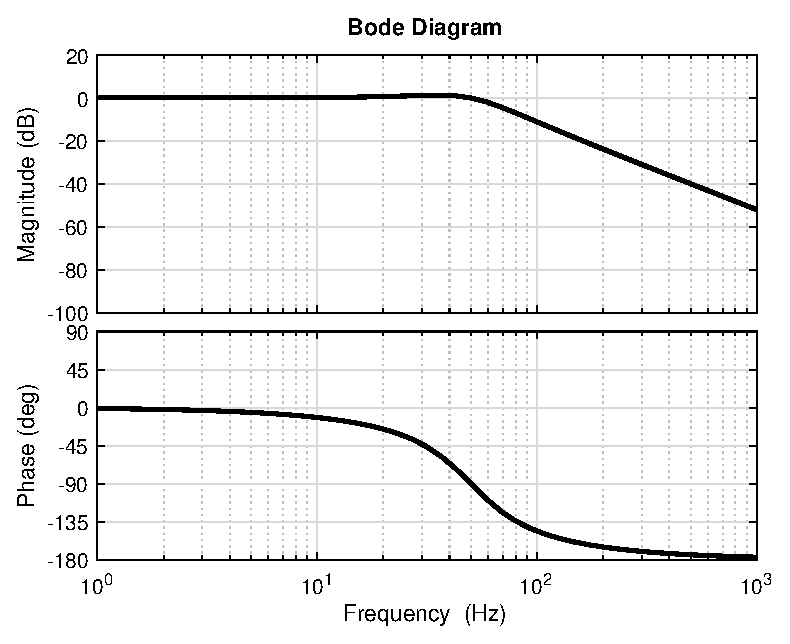
\includegraphics[width = 200pt, angle = 0,	keepaspectratio]{figures/sogi_Q(s)_bode.eps}
		\captionsetup{width=0.75\textwidth, font=footnotesize}
		\caption{Bode diagram of the $\textit{Q}(s)$ transfer function in a \textit{SOGI-QSG}.}
		\label{bode_response_Q}
	\end{subfigure}%
	\begin{subfigure}{.5\textwidth}
		\centering
		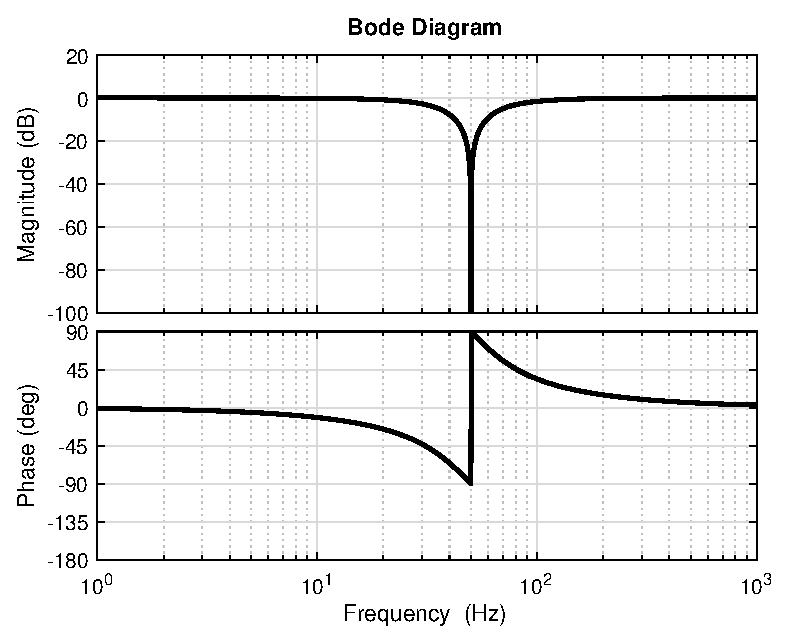
\includegraphics[width = 200pt, angle = 0,	keepaspectratio]{figures/sogi_E(s)_bode.eps}
		\captionsetup{width=0.75\textwidth, font=footnotesize}
		\caption{Bode diagram of the $\textit{E}(s)$ transfer function in a \textit{SOGI-QSG}.}
		\label{bode_response_E}
	\end{subfigure}
	\captionsetup{width=0.5\textwidth, font=small}
	\caption{Bode diagram of the \textit{SOGI-QSG} response.}
	\label{}
\end{figure}
Another useful possible implementation of the \textit{SOGI-QSG}-based \textit{PLL} is based on the direct and inverse Park transforms, as shown in Figure~\ref{park_pll_1}
\begin{figure}[H]
	\centering
	\includegraphics[width = 495pt, angle = 0, keepaspectratio]{figures/single_phase_pll_fig1b.eps}
	\captionsetup{width=0.5\textwidth, font=small}	
	\caption{PLL based on the on direct and inverse Park transform.}
	\label{park_pll_1}
\end{figure}
\begin{multicols}{2}
An equivalent transfer function block diagram is presented in Figure~\ref{park_pll_2}. In this configuration the transformation $v_\alpha\rightarrow v_\beta^{pll}$ is represented as $\omega_{pll}/s$ in Laplace domain. An intuitive explanation of its operation principle can be given if it is assumed that the \textit{PLL} is well tuned to the input signal frequency. Under such operation conditions, if $v_\alpha$ and $v_\beta^{pll}$ are not in quadrature, the virtual input vector, $v_\alpha^{pll}$, resulting from these signals will have neither constant amplitude nor rotation speed.
	\begin{figure}[H]
	\centering
	\includegraphics[width = 235pt, angle = 0, keepaspectratio]{figures/qsg_park_eq_1.eps}
	\captionsetup{width=0.35\textwidth, font=small}	
	\caption{Equivalent block diagram of the PLL based on the on direct and inverse Park transform.}
	\label{park_pll_2}
\end{figure}
 Therefore $v_\xi$ and $v_\eta$ waveform resulting from direct Park transformation will have harmonics components. These harmonics will be suppressed by the \textit{LPF} blocks generating, as well, the components $v_\xi^f$ and $v_\eta^f$. The $v_\alpha$ and $v_\beta^{pll}$ components resulting from the inverse Park transformation of the components $v_\xi^f$ and $v_\eta^f$ will be in quadrature, though $v_\alpha$ and $v_\alpha^{pll}$ will not be in phase if the \textit{PLL} is not perfectly synchronized. As the \textit{PLL} locks the phase angle of the input signal $v_\alpha$, the components $v_\alpha^{pll}$ and $v_\beta^{pll}$ will be respectively in phase and in quadrature respect to the input signal $v_\alpha$.
\end{multicols}
From the equivalent block diagram of Figure~\ref{park_pll_2} the following transfer functions can be derived
\begin{flalign}
	\boxed{\frac{V_\beta^{pll}}{V_\alpha}(s)=\frac{\omega_f\omega_{pll}}{s^2+\omega_{f}s+\omega_{pll}^2}}
\end{flalign}
\begin{flalign}
	\boxed{\frac{V_\alpha^{pll}}{V_\alpha}(s)=\frac{s\omega_f}{s^2+\omega_{f}s+\omega_{pll}^2}}
\end{flalign}
where the relation of Eq.~\eqref{alphabeta_tr_eq} has been applied.
\begin{flalign}\label{alphabeta_tr_eq}
	V_\beta^{pll}(s) = \frac{\omega_{pll}}{s}V_\alpha^{pll}(s)
\end{flalign}
%\begin{equation}
%	V_\xi(s) = \frac{1}{2}\Big[\Big(V_\alpha(s+j\omega_{pll})+V_\alpha(s-j\omega_{pll})\Big)-j\Big(V_\beta^{pll}(s+j\omega_{pll})-V_\beta^{pll}(s-j\omega_{pll})\Big)\Big]
%\end{equation}
%\begin{equation}
%	V_\eta(s) = \frac{1}{2} \Big[ j\Big(V_\alpha(s+j\omega_{pll})-V_\alpha(s-j\omega_{pll})\Big)+ \Big(V_\beta^{pll}(s+j\omega_{pll})+V_\beta^{pll}(s-j\omega_{pll})\Big)\Big]
%\end{equation}
%
%\begin{equation}
%	V_\xi^{f}(s) = \frac{\omega_{f}}{s+\omega_{f}}V_\xi(s)
%\end{equation}
%\begin{equation}
%	V_\eta^{f}(s) = \frac{\omega_{f}}{s+\omega_{f}}V_\eta(s)
%\end{equation}
%
%\begin{equation}
%	V_\xi^f(s) = \frac{1}{2}\frac{\omega_{f}}{s+\omega_{f}}\Big[\Big(V_\alpha(s+j\omega_{pll})+V_\alpha(s-j\omega_{pll})\Big)-j\Big(V_\beta^{pll}(s+j\omega_{pll})-V_\beta^{pll}(s-j\omega_{pll})\Big)\Big]
%\end{equation}
%\begin{equation}
%	V_\eta^f(s) = \frac{1}{2}\frac{\omega_{f}}{s+\omega_{f}}\Big[j\Big(V_\alpha(s+j\omega_{pll})-V_\alpha(s-j\omega_{pll})\Big)+ \Big(V_\beta^{pll}(s+j\omega_{pll})+V_\beta^{pll}(s-j\omega_{pll})\Big)\Big]
%\end{equation}
%
%\begin{equation}
%	V_\alpha^{pll}(s) = \frac{1}{2}\Big[ \Big(V_\xi^f(s+j\omega_{pll})+V_\xi^f(s-j\omega_{pll})\Big) + j\Big(V_\eta^{f}(s+j\omega_{pll})-V_\eta^{f}(s-j\omega_{pll})\Big)\Big]
%\end{equation}
%\begin{equation}
%	V_\beta^{pll}(s) = \frac{1}{2}\Big[-j\Big(V_\xi^f(s+j\omega_{pll})-V_\xi^f(s-j\omega_{pll})\Big) + \Big(V_\eta^{f}(s+j\omega_{pll})+V_\eta^{f}(s-j\omega_{pll})\Big)\Big]
%\end{equation}

\begin{figure}[H]
	\centering
	\begin{subfigure}{.5\textwidth}
		\centering
		\includegraphics[width = 200pt, angle = 0,	keepaspectratio]{figures/Hin.eps}
		\captionsetup{width=0.75\textwidth, font=footnotesize}
		\caption{Bode diagram of the $\frac{V_\alpha^{pll}}{V_\alpha}(s)$ transfer function, with $\omega_f=2\pi\SI{50}{\hertz}$, and $\omega_{pll}=2\pi\SI{400}{\hertz}$.}
		\label{}
	\end{subfigure}%
	\begin{subfigure}{.5\textwidth}
		\centering
		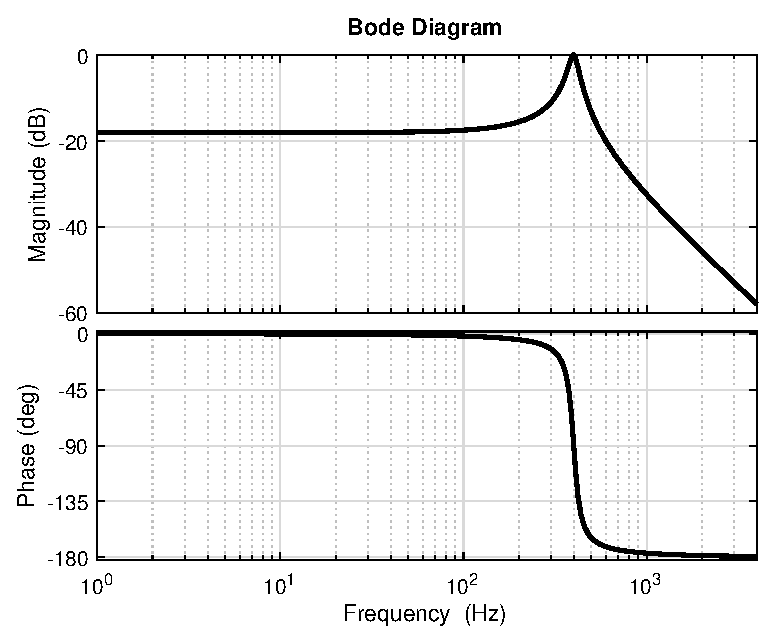
\includegraphics[width = 200pt, angle = 0,	keepaspectratio]{figures/Hq.eps}
		\captionsetup{width=0.75\textwidth, font=footnotesize}
		\caption{Bode diagram of the $\frac{V_\beta^{pll}}{V_\alpha}(s)$ transfer function, with $\omega_f=2\pi\SI{50}{\hertz}$, and $\omega_{pll}=2\pi\SI{400}{\hertz}$.}
		\label{}
	\end{subfigure}
	\captionsetup{width=0.5\textwidth, font=small}
	\caption{Bode diagram of the \textit{QSG-PLL} based on direct and inverse Parck transform.}
	\label{}
\end{figure}
%\begin{equation*}
%	\begin{aligned}
%		V_\alpha^{pll}(s) &= \frac{1}{2}\Big\{\frac{1}{2}\frac{\omega_{f}}{s+\omega_{f}}\Big[\Big(V_\alpha(s+2j\omega_{pll})+V_\alpha(s)\Big)-j\Big(V_\beta^{pll}(s+2j\omega_{pll})-V_\beta^{pll}(s)\Big)\Big] + \\[6pt]
%	&\quad+\frac{1}{2}\frac{\omega_{f}}{s+\omega_{f}}\Big[\Big(V_\alpha(s)+V_\alpha(s-2j\omega_{pll})\Big)-j\Big(V_\beta^{pll}(s)-V_\beta^{pll}(s-2j\omega_{pll})\Big)\Big] + \\[6pt]
%	&\quad+j\frac{1}{2}\frac{\omega_{f}}{s+\omega_{f}}\Big[j\Big(V_\alpha(s+2j\omega_{pll})-V_\alpha(s)\Big)+ \Big(V_\beta^{pll}(s+2j\omega_{pll})+V_\beta^{pll}(s)\Big)\Big]+ \\[6pt]
%	&\quad-j\frac{1}{2}\frac{\omega_{f}}{s+\omega_{f}}\Big[j\Big(V_\alpha(s)-V_\alpha(s-2j\omega_{pll})\Big)+ \Big(V_\beta^{pll}(s)+V_\beta^{pll}(s-2j\omega_{pll})\Big)\Big]\Big\}
%	\end{aligned}
%\end{equation*}
%
%\begin{equation*}
%	\begin{aligned}
%		V_\beta^{pll}(s) &= \frac{1}{2}\Big\{-j\frac{1}{2}\frac{\omega_{f}}{s+\omega_{f}}\Big[\Big(V_\alpha(s+2j\omega_{pll})+V_\alpha(s)\Big)-j\Big(V_\beta^{pll}(s+2j\omega_{pll})-V_\beta^{pll}(s)\Big)\Big] + \\[6pt]
%		&\quad+j\frac{1}{2}\frac{\omega_{f}}{s+\omega_{f}}\Big[\Big(V_\alpha(s)+V_\alpha(s-2j\omega_{pll})\Big)-j\Big(V_\beta^{pll}(s)-V_\beta^{pll}(s-2j\omega_{pll})\Big)\Big] + \\[6pt]
%		&\quad+\frac{1}{2}\frac{\omega_{f}}{s+\omega_{f}}\Big[j\Big(V_\alpha(s+2j\omega_{pll})-V_\alpha(s)\Big)+ \Big(V_\beta^{pll}(s+2j\omega_{pll})+V_\beta^{pll}(s)\Big)\Big]+ \\[6pt]
%		&\quad+\frac{1}{2}\frac{\omega_{f}}{s+\omega_{f}}\Big[j\Big(V_\alpha(s)-V_\alpha(s-2j\omega_{pll})\Big)+ \Big(V_\beta^{pll}(s)+V_\beta^{pll}(s-2j\omega_{pll})\Big)\Big]\Big\}
%	\end{aligned}
%\end{equation*}

\chapter{Moving Average Filter}	

\section{Basic Idea of the Moving Average Filter}
The moving average (MAVG) filter is used, in this contest, to calculate the average value of a periodic waveform. The basic consist of to sample the whole period of the waveform and calculate the mean value according to
\begin{equation}\label{mavg_flt_eq_1}
	x_m(k)=\frac{1}{N}\sum_{i=0}^{N-1}x(k-i)
\end{equation}
\begin{figure}[H]
	\centering
	\includegraphics[width = 325pt, angle = 0, 
	keepaspectratio]{figures/mavg_flt_fig_2.eps}
	\captionsetup{width=0.5\textwidth, font=small}
	\caption{Principle of the moving average filter.}
	\label{mavg_flt_fig_1}
\end{figure}
Representing Eq.~\eqref{mavg_flt_eq_1} with the $\mathscr{Z}$-transform, it results
\begin{equation}\label{mavg_flt_eq_2}
	X_m(z)=\frac{1}{N}\mathscr{Z}\Bigg[\sum_{i=0}^{N-1}x(k-i)\Bigg] = \frac{1}{N}X(z)\sum_{i=0}^{N-1}z^{-i}=\frac{1}{N}X(z)\frac{1-z^{-N}}{1-z^{-1}}
\end{equation}
The term $X_s(z)=X(z)\frac{1-z^{-N}}{1-z^{-1}}$ represents the summation of the $x(k)$ samples along a window period of $N$-samples. the mean value of the $x(k)$ signal results, in the $\mathscr{Z}$-transform domain,
\begin{equation}\label{mavg_flt_eq_3}
 	X_m(z)=\frac{1}{N}X_s(z)
\end{equation}
the representation of the term $X_s(z)=X(z)\frac{1-z^{-N}}{1-z^{-1}}$ into the discrete time domain results as follows
\begin{equation}\label{mavg_flt_eq_4}
	x_s(k)=	x_s(k-1)+x(k)-x(k-N)
\end{equation}
and the mean value of the $x(k)$ signal results, along a window period of $N$-samples,
\begin{equation}\label{mavg_flt_eq_5}
	x_m(k)=	\frac{1}{N}x_s(k)
\end{equation}
From an implementation point of view Eq.~\eqref{mavg_flt_eq_4} shall be divided into two equations:
\begin{flalign}
		x_s(k) &= x_s(k-1)+x(k)\qquad \text{\footnotesize until the buffer of $N$-elements is not yet loaded} \label{mavg_flt_eq_6} \\[6pt]
		x_s(k) &= x_s(k-1)+x(k)-x(k-N)\qquad \text{\footnotesize when the buffer of $N$-elements is already loaded} \label{mavg_flt_eq_7}
\end{flalign}
Define $\omega$ the pulsation of input signal $x(t)$ and $t_s$ the sampling time of the \textit{MAVG} filter. An important aspect concerning the performance of the \textit{MAVG} filter lays when an integer number of sampling time $t_s$ doesn't cover perfectly the period ($2\pi/\omega$) of the input signal. In this case exist a technique which is able to overcome the error occurred when the buffer doesn't cover perfectly the period of the input signal. The algorithm consists of to implement two \textit{MAVG} filter with different buffer windows, respectively with\footnote{Consider that the function $\text{int}()\equiv\text{floor}()$}
\begin{flalign}
	N_\text{inf} &= \text{int}\Bigg(\frac{2\pi}{\omega t_s}\Bigg) \label{mavg_flt_eq_8} \\[6pt]
	N_\text{sup} &= \text{int}\Bigg(\frac{2\pi}{\omega t_s}\Bigg)+1 \label{mavg_flt_eq_9}
\end{flalign}
\begin{figure}[H]
	\centering
	\includegraphics[width = 395pt, angle = 0, 
	keepaspectratio]{figures/mavg_flt_fig_3b.eps}
	\captionsetup{width=0.5\textwidth, font=small}
	\caption{Algorithm description for not integer $t_s$ overlapping of the signal period.}
	\label{mavg_flt_fig_2}
\end{figure}
the two average quantities will be summed with the relative weight, as follows (see also Figure~\ref{mavg_flt_fig_2})
\begin{flalign}
	x_m(k) = \zeta x_m^{\text{inf}}+\big(1-\zeta\big)x_m^{\text{sup}}
\end{flalign}
where 
\begin{flalign}
	\zeta = \frac{2\pi}{\omega t_s}-\text{int}\Bigg(\frac{2\pi}{\omega t_s}\Bigg)
\end{flalign}
\section{Buffer Management of the Moving Average Filter}	
An important aspect for the implementation of an efficient \textit{MAVG} filter is the management of the buffer used to calculate the average value of the input signal. According to Figure~\ref{mavg_flt_fig_3} the buffer used for the \textit{MAVG} can be considered a FIFO. To access to the buffer data it is necessary to consider two case:
\begin{itemize}
	\item[--] the current buffer index $i$ is greater than the offset window ($N$);
	\begin{equation}
		i_N=i-d
	\end{equation}
	\item[--] the current buffer index $i$ is less than the offset window ($N$)
	\begin{equation}
		i_N=i-d+N_\text{max}
	\end{equation}
\end{itemize}
where $N_\text{max}$ is the size of the buffer.
\begin{figure}[H]
	\centering
	\includegraphics[width = 400pt, angle = 0, 
	keepaspectratio]{figures/buffer_management_fig1.eps}
	\captionsetup{width=0.5\textwidth, font=small}
	\caption{Buffer management of the moving average filter.}
	\label{mavg_flt_fig_3}
\end{figure}
The buffer size shall be selected according to the maximum period of the input signal
\begin{equation}
	N_\text{max}=\frac{2\pi}{\omega_\text{min}t_s}
\end{equation}

\section{C-code Implementation}
The moving average filter has been implemented in the \textit{Simulink} model as \textit{Custom Code} by the \textit{C-Caller}\footnote{C-Caller is used to integrate user C-code in Simulink}.

The code structure is composed by four files:
\begin{itemize}
	\item[--] {\fontfamily{cmss}\selectfont \verb+mavgflt_simulink.h+}: the file structure data for the structure for the interface between the \textit{Simulink} model and the inner custom code.
	\item[--] {\fontfamily{cmss}\selectfont \verb+mavgflt.h+}: the file include structure data and header functions for the \textit{MAVG} filter
	\item[--] {\fontfamily{cmss}\selectfont \verb+mavgflt_simulink.c+}: the file include the source code for the interface between the \textit{Simulink} model and the inner custom code.
\item[--] {\fontfamily{cmss}\selectfont \verb+mavgflt.c+}: the file include source code functions for the \textit{MAVG} filter
\end{itemize}	
\begin{mybox}
\begin{center}
	{\fontfamily{cmss}\selectfont \verb+mavgflt_simulink.h+}
\end{center}
{\fontfamily{cmss}\selectfont \footnotesize \noindent
	\begin{verbatim}
		#ifndef   _MAVGFLT_SIMULINK_
		#define   _MAVGFLT_SIMULINK_
		#define    NMAVGFLT_INSTANCES  16

		typedef struct mavgflt_output_s {
			float ts;                   /*sampling time*/
			float sshort;               /*sum short (N-1 samples)*/
			float slong;                /*sum long (N samples)*/
			float pinput;               /*previous input*/
			unsigned int cbpointer;     /*current buffer pointer*/
			unsigned int cbsample;      /*current buffer sample*/
			float mavg_output;          /*moving average filter output*/
		} mavgflt_output_t;
	
		#define MAVGFLT_OUTPUT mavgflt_output_t
	
		MAVGFLT_OUTPUT mavgflt_process_simulink(const float input, const float period, const float ts, 
		unsigned char reset, unsigned char instance);
		#endif
	\end{verbatim}}
\end{mybox}

\begin{mybox}
\begin{center}
	{\fontfamily{cmss}\selectfont \verb+mavgflt.h+}
\end{center}
{\fontfamily{cmss}\selectfont \footnotesize \noindent
	\begin{verbatim}
#ifndef _MAVGFLT_
#define _MAVGFLT_
#define MAVGFLT_SIZE        152
#define MAVGFLT_SIZE_MIN    78
#define MAVGFLT_SIZE_MAX    420

typedef struct mavgflt_s {
	float ts;                          /*Filter time base.*/
	float sshort;                      /*Integration with floor period length.*/
	float slong;                       /*Integration with ceil period length.*/
	float pinput;                      /*step back input value*/
	float buffer[MAVGFLT_SIZE_MAX];    /*buffer*/
	unsigned int cbpointer;            /*buffer array pointer for the newest element to be written*/
	unsigned int cbsample;             /*current number of samples for the current period*/
} mavgflt_t;

#define MAVGFLT mavgflt_t

void mavgflt_init(volatile MAVGFLT *f);
void mavgflt_ts(volatile MAVGFLT *f, volatile float ts);
void mavgflt_reset(volatile MAVGFLT *f);
float mavgflt_process(volatile MAVGFLT *f, float input, const float period);
#endif
\end{verbatim}}
\end{mybox}

\begin{mybox}
\begin{center}
	{\fontfamily{cmss}\selectfont \verb+mavgflt_simulink.c+}
\end{center}
{\fontfamily{cmss}\selectfont \footnotesize \noindent
	\begin{verbatim}
	#include <include/mavgflt.h>
	#include <include/mavgflt_simulink.h>
	static void init_allmavgflt_instances(MAVGFLT *const filter_list, const unsigned int filter_num)
	{
	    unsigned int i;
	    for (i = 0; i < filter_num; ++i) {
	        MAVGFLT *const filter = &filter_list[i];
	        mavgflt_init(filter);
            i++;
	    }
	}
	MAVGFLT_OUTPUT mavgflt_process_simulink(const float input, const float period, const float ts, 
	unsigned char reset, unsigned char instance)
	{
	    static MAVGFLT filter_instances[NMAVGFLT_INSTANCES] = {0};
	    static unsigned int filter_initialized = 0;
	    if (!filter_initialized){
	        init_allmavgflt_instances(filter_instances, NMAVGFLT_INSTANCES);
            filter_initialized = 1;
		}
		if (instance < NMAVGFLT_INSTANCES) {
		    const MAVGFLT* filter_instance = &filter_instances[instance];
		    mavgflt_ts(filter_instance, ts);
		    if(reset)
		    {
		        mavgflt_reset(filter_instance);
		    }
		    const float output_value = mavgflt_process(filter_instance, input, period);
		    const MAVGFLT_OUTPUT filter_output = {
		        .ts = filter_instance->ts,
		        .sshort = filter_instance->sshort,
		        .slong = filter_instance->slong,
		        .pinput = filter_instance->pinput,
		        .cbpointer = filter_instance->cbpointer,
		        .cbsample = filter_instance->cbsample,
		        .mavg_output = output_value
		    };
		    return filter_output;
		}
		else{
		    const MAVGFLT_OUTPUT empty_output = {0};
	        return empty_output;
	    }
	}
	\end{verbatim}}
\end{mybox}

\begin{mybox}
\begin{center}
	{\fontfamily{cmss}\selectfont \verb+mavgflt.c+}
\end{center}
{\fontfamily{cmss}\selectfont \footnotesize \noindent
	\begin{verbatim}
#include <include/mavgflt.h>
void mavgflt_init(volatile MAVGFLT *f)
{
    f->ts = 0.0;
    mavgflt_reset(f);
}
void mavgflt_ts(volatile MAVGFLT *f, volatile float ts)
{
    f->ts = ts;
}
void mavgflt_reset(volatile MAVGFLT *f)
{
    int i;
    f->pinput = 0.0;
    f->sshort = 0.0;
    f->slong = 0.0;
    f->cbpointer = 0;
    f->cbsample = 0;
    for (i = 0; i < MAVGFLT_SIZE_MAX; i++) {
        f->buffer[i] = 0.0;
    }
}
static unsigned int get_buffer_pointer(const unsigned int cbpointer, const unsigned int cnperiod)
{
    if (cnperiod <= cbpointer) {
        return cbpointer - cnperiod;
    }
    else {
        return cbpointer - cnperiod + MAVGFLT_SIZE_MAX;
    }
}
static float get_buffer_value(const MAVGFLT * const f, const unsigned int cnperiod)
{
    const unsigned int current_nperiod = get_buffer_pointer(f->cbpointer, cnperiod);
    return f->buffer[current_nperiod];
}
float mavgflt_process(volatile MAVGFLT *f, float input, const float period)
{
    if (period > 0.0) {
        float samples_requested_f = period / f->ts;
        if (samples_requested_f > MAVGFLT_SIZE_MAX - 1)
        samples_requested_f = MAVGFLT_SIZE_MAX - 1;
        const unsigned int cnbuffer = samples_requested_f + 1;
        const float sampling_fraction = samples_requested_f + 1 - cnbuffer;
        if (cnbuffer > f->cbsample) {
            f->sshort += f->pinput;
            f->slong += input;
            f->cbsample++;
        }
        else if (cnbuffer < f->cbsample) {
            const unsigned int decremented_cbsample = f->cbsample - 1;
            const float two_oldest_samples = get_buffer_value((MAVGFLT*) f, f->cbsample)
            + get_buffer_value((MAVGFLT*) f, decremented_cbsample);
            f->sshort += f->pinput - two_oldest_samples;
            f->slong += input - two_oldest_samples;
            f->cbsample = decremented_cbsample;
        }
        else {
            const float oldest_period_sample = get_buffer_value((MAVGFLT*) f, f->cbsample);
            f->sshort += f->pinput - oldest_period_sample;
            f->slong += input - oldest_period_sample;
        }
        f->buffer[f->cbpointer] = input;
        f->cbpointer++;
        f->pinput = input;
        if (f->cbpointer == MAVGFLT_SIZE_MAX) {
            f->cbpointer = 0;
        }
        const float cbsample_short = f->cbsample - 1;
        const float filter_output_short = cbsample_short ? f->sshort / cbsample_short : 0.0;
        const float filter_output_long = f->slong / f->cbsample;
        return filter_output_short * (1 - sampling_fraction) + 
        filter_output_long * sampling_fraction;
    }
    else {
        return 0.0;
    }
}
\end{verbatim}}
\end{mybox}

	
\chapter{Implementation on dSPACE SCALEXIO}	
\section{Introduction}
The theory of the \textit{PLL} and of the \textit{MAVG} filter described along the previous chapters will be experimentally investigated using the fast prototyping equipment \textit{SCALEXIO}. The structure of the experiment is depicted in Figure~\ref{scalexio_fig_2}. 
\begin{figure}[H]
	\centering
	\includegraphics[width = 320pt, angle = 0, 
	keepaspectratio]{figures/scalexio/hardware_config_2.eps}
	\captionsetup{width=0.5\textwidth, font=small}
	\caption{Description of the experiment.}
	\label{scalexio_fig_2}
\end{figure}
Conceptually the experiment consists of to generate a signal from the scalexio box and to loop it back into the scalexio itself where the \textit{PLL} application is applied. The loop back will be implemented by an analog output and an analog input available on DS6101 board of the scalexio.

Via Simulink an application of the \textit{PLL} and of the \textit{MAVG} filter is designed as well as a signal generator. The output of the signal generator is connected to an analog voltage output of the \textit{SCALEXIO}. The analog voltage output is looped back to an analog voltage input of the \textit{SCALEXIO} and it is used as signal input to the \textit{PLL} and \textit{MAVG} filter application. The analog voltage input and output are taken from the DS6101 board available on the \textit{SCALEXIO} according Figure~\ref{scalexio_fig_1}. The connection between Simulink model and the scalexio I/O will activated via \textit{ConfigurationDesk} during the phase of creation of the project.

\section{Configuring the experiment}
In this section the configuration of the project/experiment on \textit{ConfigurationDesk} is shown. Figure~\ref{scalexio_fig_1} shows the hardware and model interface structure which must be implemented in the \textit{ConfigurationDESK} application.
\begin{figure}[H]
	\centering
	\includegraphics[width = 495pt, angle = 0, 
	keepaspectratio]{figures/scalexio/hardware_config_1.eps}
	\captionsetup{width=0.5\textwidth, font=small}
	\caption{Hardware configuration of the experiment.}
	\label{scalexio_fig_1}
\end{figure}
Supposing to be in the \textit{ConfigurationDESK} application and to have already created and loaded the application:
\begin{itemize}
	\item[--] from \textit{signal chain} drag and drop the \textit{Analog In 4 - Channel 1} from \textit{Hardware Resource} to \textit{Global/Signal Chain} window;
	\item[--] again, drag and drop the \textit{Analog Out 7 - Channel 1} from \textit{Hardware Resource} to \textit{Global/Signal Chain} window;
	\item[--] select \textit{Voltage In (1)} and RMB and select \textit{Propagate to ConfigurationDesk Model Interface};
	\item[--] select \textit{Voltage In (1)} and RMB and select \textit{Propagate to ConfigurationDesk Model Interface};
\end{itemize}
Now in the \textit{Model Port Blocks} of the \textit{Signal Chain} window the are to additional blocks which are the interface between the scalexio device and the simulink model.
\begin{itemize}
	\item[--] from \textit{signal chain} RMB on \textit{Voltage In (1)} and select \textit{Propagate to Simulink Model};
	\item[--] from \textit{signal chain} RMB on \textit{Voltage Out (1)} and select \textit{Propagate to Simulink Model};
\end{itemize}
Now two additional interface \textit{dSPACE} blocks shall be available in the simulink model, \textit{Voltage - Data Inport Block} and \textit{Voltage - Data Outport Block} respectively.

The creation of the \textit{external device} can be done in two different ways:
\begin{itemize}
	\item[--] from \textit{External Devices} available on the left window of the \textit{Signal Chain} tab RMB and \textit{Import Devices} (merge/replace). The external device can be imported as file \textit{*.dtfx} file;
	\item[--] the external device can be created directly from \textit{External Devices} tab available on the left window of the \textit{Signal Chain} tab, see the Section~\ref{creating_new_hardware}.
\end{itemize}

After the connection of the blocks, which must be done according to the purpose of the project, the \textit{Signal Chain} window will appear similarly to Figure~\ref{scalexio_fig_1}.

\section{Creating the external hardware}\label{creating_new_hardware}
The external device interface can be created from the \textit{External Devices} tab of the left window of the \textit{Signal Chain} tab of the \textit{ConfigurationDesk}, as follows:
\begin{itemize}
	\item[--] from \textit{External Devices} tab, available on the left window of the \textit{Signal Chain} tab RMB and select \textit{New/Device}. Suppose to rename it: \textit{Loop\_back};
	\item[--] RMB on \textit{Loop\_back} new device and select \textit{New/Port} and rename it, e.g.: \textit{Voltage\_in\_GND};
	\item[--] select the \textit{Voltage\_in\_GND} port and update information on \textit{Electrical Interface} available of the right window of the \textit{Signal Chain} tab;
		\begin{itemize}
		\item[--] from \textit{Electrical Interface} select \textit{Device Port Settings/Port Type} and select \textit{In};
		\item[--] from \textit{Electrical Interface} select \textit{Device Port Settings/Port Attributes} and select \textit{Voltage};
		\end{itemize}
	\item[--] RMB on \textit{Loop\_back} new device and select \textit{New/Port} and rename it, e.g.: \textit{Voltage\_in\_SIGNAL};
	\item[--] select the \textit{Voltage\_in\_SIGNAL} port
		\begin{itemize}
			\item[--] from \textit{Electrical Interface} select \textit{Device Port Settings/Port Type} and select \textit{In};
			\item[--] from \textit{Electrical Interface} select \textit{Device Port Settings/Port Attributes} and select \textit{Voltage};
		\end{itemize}
	\item[--] RMB on \textit{Loop\_back} new device and select \textit{New/Port} and rename it, e.g.: \textit{Voltage\_out\_GND};
	\item[--] select the \textit{Voltage\_out\_GND} port
		\begin{itemize}
			\item[--] from \textit{Electrical Interface} select \textit{Device Port Settings/Port Type} and select \textit{Out};
			\item[--] from \textit{Electrical Interface} select \textit{Device Port Settings/Port Attributes} and select \textit{Voltage};
		\end{itemize}
	\item[--] RMB on \textit{Loop\_back} new device and select \textit{New/Port} and rename it, e.g.: \textit{Voltage\_out\_SIGNAL};
		\item[--] select the \textit{Voltage\_out\_SIGNAL} port
		\begin{itemize}
			\item[--] from \textit{Electrical Interface} select \textit{Device Port Settings/Port Type} and select \textit{Out};
			\item[--] from \textit{Electrical Interface} select \textit{Device Port Settings/Port Attributes} and select \textit{Voltage};
		\end{itemize}	
\end{itemize}


\chapter{Appendices}	
\section{The Fourier Series}



\begin{thebibliography}{99}
	% power electronics
	\bibitem{liserre} 
	R. Teodorescu, M. Liserre, P. Rodrıguez, \emph{Grid converters for photovoltaic and wind power systems}. Wiley, 2011.
\end{thebibliography}

\end{document} 